\section{Results}
\label{sec:results}

\paragraph{Reading guide.}
Primary numbers use locked $R_{\mathrm{blend}}$ (Sections~\ref{sec:v10-freeze}--\ref{sec:n2n-vs-ours-boards}).
Hard-cliff classical collapse and multi-family ranking follow.
Matched outer-loop bake-offs, HP probes, branch freezes, and transfer latency sit in Appendix~\ref{app:supplement}.
Honesty notes are collected in Section~\ref{sec:limitations}.

\begin{figure}[t]
  \centering
  
\includegraphics[width=\columnwidth]{figures/fig_meta_heal_samples.png}
  \caption{Holdout wrap-seam heal for the hybrid champion vs no-bake, Dual Cosine, and ideal sibling $r^{\star}$ (seed \texttt{20260719}).}
  \label{fig:meta-heal-samples}
\end{figure}

\subsection{Hybrid search under the blended score}
\label{sec:v10-freeze}
Does hybrid GA+PPO beat the frozen Noise2Noise gate under $R_{\mathrm{blend}}$ and $J$?
A $1{,}200$-iteration search (seed \texttt{1902771841}, ${\approx}1.65$\,h wall) selects on
$J$~\eqref{eq:outer-obj} ($\lambda{=}0.02$).
Champion: $R_{\mathrm{blend}}{\approx}0.9695$, $J{\approx}0.9603$, $t{\approx}5.08$\,ms.
Search-monitor Dual Cosine on the same runner: $R_{\mathrm{blend}}{\approx}0.504$.
Frozen Noise2Noise holdout gate: $R_{\mathrm{blend}}{\approx}0.9750$.
The search champ does \emph{not} clear that gate, while clearly clearing Dual Cosine.
Artifacts: \href{https://github.com/reeldemo/denoise-opt-meta/blob/master/paper/Unsupervised_Wrap-Discontinuity_Repair_in_Wavetable_Synthesis_via_Hybrid_GA-PPO_Meta-Search_v12/figures/meta_approach_compare_v10.json}{hybrid search data}.

\subsection{Noise2Noise vs Ours on four boards}
\label{sec:n2n-vs-ours-boards}
Table~\ref{tab:n2n-vs-ours} summarizes the four evaluation boards under $R_{\mathrm{blend}}$,
with Dual Cosine as the classical fade row on every board.
On the frozen sine{+}cliff holdout (seed \texttt{20260719}), Noise2Noise leads Ours
($0.9750$ vs $0.9697$, $\Delta{\approx}{-}0.0053$), while Dual Cosine collapses to $0.5409$
(Ours$-$DualCosine $\Delta{\approx}{+}0.429$).
On the $20$-waveform multi-family board, Ours mean $0.9311$ exceeds N2N $0.9249$
($13/20$ wins, $\Delta$ mean ${\approx}{+}0.0062$) and both dominate Dual Cosine (mean ${\approx}0.514$).
On balanced wavetable-native corpora ($n{=}1{,}280$ each), N2N leads Factory+FX
($0.771$ vs Ours $0.699$, Dual Cosine $0.589$) and AKWF
($0.731$ vs Ours $0.679$, Dual Cosine $0.424$).
Latency: holdout Ours ${\approx}4.57$\,ms vs N2N ${\approx}0.65$\,ms ($J$ still favors N2N on holdout).

\begin{table}[t]
  \centering
  \caption{Parameter-count fairness under the locked holdout story.
    Favorite $\Theta$ is the v10.1 hybrid champion cell (search seed \texttt{1902771841}).
    SeamN2N is the frozen corrupt$\to$corrupt gate (train seed \texttt{424242}).}
  \label{tab:param-fairness}
  \setlength{\tabcolsep}{4pt}
  \begin{tabular}{@{}lrr@{}}
    \toprule
    Method & Params & Holdout $R_{\mathrm{blend}}$ \\
    \midrule
    Favorite $\Theta$ (v10.1 hybrid) & ${\approx}121$k & $0.9697$ \\
    SeamN2N (corrupt$\to$corrupt) & ${\approx}53.5$k & $0.9750$ \\
    Dual Cosine & $0$ & $0.5409$ \\
    \bottomrule
  \end{tabular}
\end{table}

\noindent
Table~\ref{tab:param-fairness} states the size comparison the review requested.
The hybrid favorite is larger than SeamN2N on this freeze.
N2N still leads holdout $R_{\mathrm{blend}}$.
Search seed \texttt{1902771841}, N2N train seed \texttt{424242}, and holdout seed \texttt{20260719} stay disjoint.

\paragraph{Variance honesty.}
Where multi-seed boards already exist, we report mean$\pm$std
(Table~\ref{tab:canonical-methods} five-seed prolonged-$R$ snapshot; Table~\ref{tab:sota-main} twenty-waveform $\pm$).
The primary four-board Table~\ref{tab:n2n-vs-ours} is a single locked freeze per board under DAFx/AES reporting norms.
We do not invent error bars for single-run boards.

\subsection{Search efficiency (learning curves)}
\label{sec:search-learning-curve}
Champion score versus outer-loop evaluation index is plotted in Figure~\ref{fig:search-learning-curve}.
The left panel compares a matched $5{,}000$-evaluation hybrid to Random NAS under \emph{superseded} whole-curve prolonged $R$ (seed \texttt{1902771841}, Dual Cosine ${\approx}0.817$), where both arms clear Dual Cosine early.
The right panel is different.
Under locked $R_{\mathrm{blend}}$ / $J$ over $1{,}200$ evaluations, raw champion $R_{\mathrm{blend}}$ clears Dual Cosine immediately and plateaus below the Noise2Noise gate (${\approx}0.975$), and no Random NAS curve under $R_{\mathrm{blend}}$ appears in the released logs (Deferred D1 / \texttt{METRIC\_REGEN.md}).
Plateau boredom retunes branch mix (Section~\ref{sec:hybrid}).
Near-ceiling residuals climb only a little after the first few hundred evaluations.

\begin{figure*}[t]
  \centering
  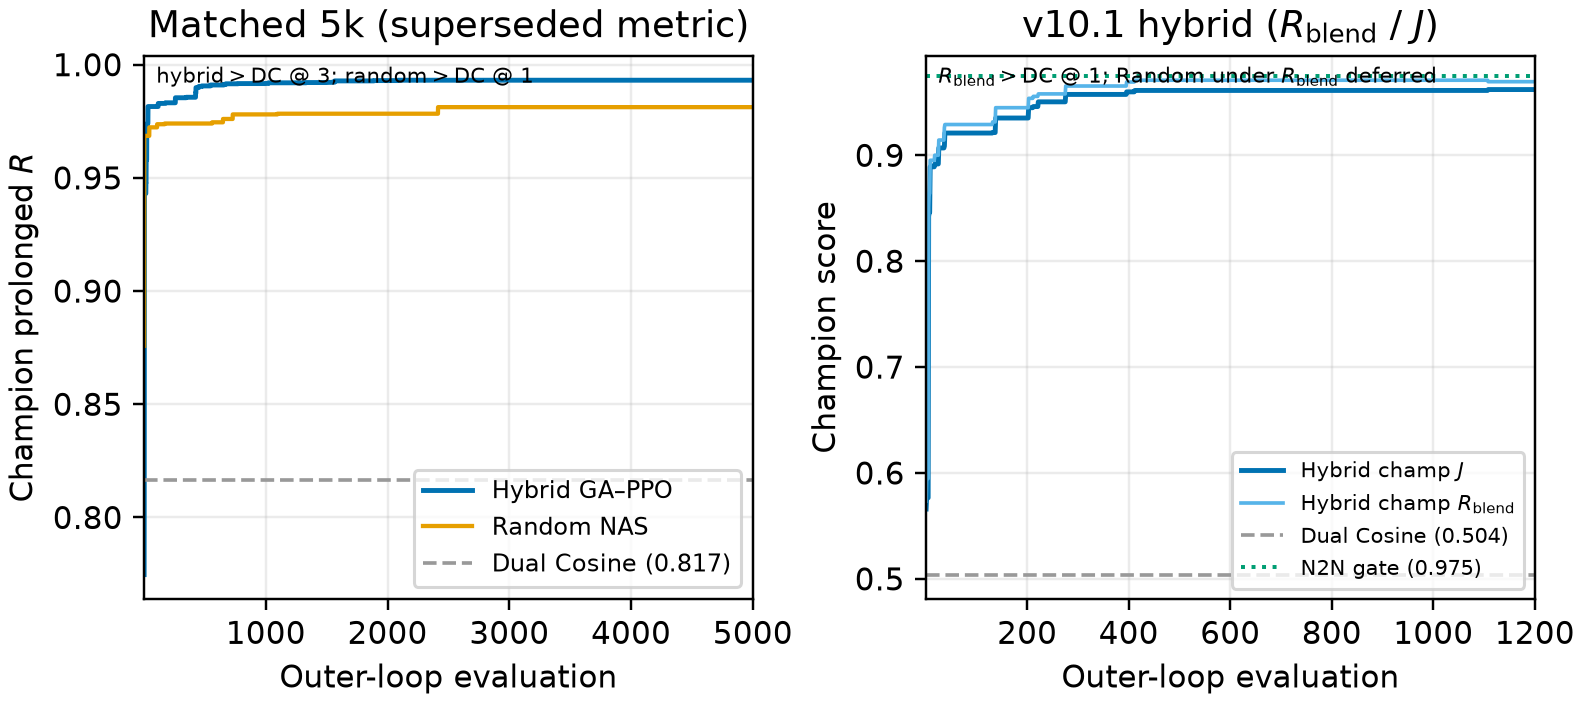
\includegraphics[width=\textwidth]{figures/fig_search_learning_curve.png}
  \caption{Search learning curves (seed \texttt{1902771841}).
    Left: champion prolonged $R$ for hybrid GA--PPO vs Random NAS on the matched $5$k bake-off
    (\textbf{superseded} whole-curve metric; Dual Cosine dashed).
    Right: v10.1 hybrid champion $J$ and raw $R_{\mathrm{blend}}$ over $1{,}200$ evaluations
    (Dual Cosine and Noise2Noise gate marked; Random under $R_{\mathrm{blend}}$ deferred).}
  \label{fig:search-learning-curve}
\end{figure*}

\begin{table}[t]
  \centering
  \caption{Ours vs Noise2Noise and Dual Cosine under $R_{\mathrm{blend}}$ ($\alpha{=}0.7$).
    $\Delta$ columns are Ours minus that baseline. Gate: Ours exceeds N2N.}
  \label{tab:n2n-vs-ours}
  \footnotesize
  \setlength{\tabcolsep}{2pt}
  \begin{tabular}{@{}lrrrrrc@{}}
    \toprule
    Board & Ours & N2N & DualCosine & $\Delta_{\mathrm{N2N}}$ & $\Delta_{\mathrm{DC}}$ & Gate \\
    \midrule
    Holdout & 0.9697 & 0.9750 & 0.5409 & $-0.0053$ & $+0.4289$ & no \\
    Multi-family (mean) & 0.9311 & 0.9249 & 0.5144 & $+0.0062$ & $+0.4167$ & $13/20$ \\
    Factory+FX & 0.6990 & 0.7714 & 0.5887 & $-0.0724$ & $+0.1104$ & no \\
    AKWF OA & 0.6794 & 0.7305 & 0.4244 & $-0.0511$ & $+0.2551$ & no \\
    \bottomrule
  \end{tabular}
\end{table}

\paragraph{Superseded whole-curve freezes.}
Whole-curve prolonged-$R$ freezes ($R{\approx}0.991$ vs DualCosine ${\approx}0.825$) are not current results.
Selection and published comparison under v10.1 use $R_{\mathrm{blend}}{+}J$ with Noise2Noise as the primary neural baseline.
Boards still carrying only prolonged $R$ need regeneration under $R_{\mathrm{blend}}$ (Limitations).

\subsection{Which families stay hard}
\label{sec:family-hardness}
On the fitted DenoiseOpt $100{,}000$-cycle bench, denoise score $D$ is lowest for \texttt{nonlinear} ($D\approx 0.39$) and \texttt{combo} ($D\approx 0.40$), then \texttt{triple\_mix} / \texttt{extreme\_overlay} ($D\approx 0.51$--$0.52$), while \texttt{harmonic\_fft} and \texttt{am\_fm} sit near $D\approx 0.69$--$0.70$.
Lit-combo champion family stress (prolonged residual) similarly ranks \texttt{open\_wrap\_bias} ($R\approx 0.83$) and \texttt{extreme\_overlay} / \texttt{combo} ($R\approx 0.88$--$0.89$) below \texttt{harmonic\_fft} ($R\approx 0.95$).
Hard sounds recur.

\paragraph{Superseded $5$k-gate freeze.}
At the reported $5$k-gate search freeze ($\approx 6{,}922$ clean iterations, $\approx 7.9$\,h on RTX~3090) the champion residual was $R\approx 0.99093$ with DualCosine $\approx 0.81658$ on the CUDA search runner ($\Delta R\approx{+}0.174$).
That freeze optimized whole-curve prolonged $R$.
It is superseded by $R_{\mathrm{blend}}$ for v10.1 selection.
Monitoring plots below come from that older freeze and should be read as search-trace artifacts, not as locked-protocol scores.

\subsection{Inference latency at matched score}
\label{sec:inference-latency}
Across the prior high-prolonged-$R$ fitted operators, we re-timed CUDA forward passes under locked $R_{\mathrm{blend}}$ (batch 64).
Live $R_{\mathrm{blend}}$ spreads more than the old prolonged band: the max-$R_{\mathrm{blend}}$ model is
\texttt{champion\_iter\_000265} ($R_{\mathrm{blend}}{\approx}0.9769$, $\approx 6.53$\,ms/batch, $\approx 94$k params).
The compact historically favorite \texttt{iter\_000235} remains lowest-latency among the top-5 distinct topologies
($R_{\mathrm{blend}}{\approx}0.9749$, $\approx 3.42$\,ms/batch, $\approx 37$k params).
Selection rule: maximize live $R_{\mathrm{blend}}$, then minimize latency inside $R\ge R_{\max}-5\cdot10^{-4}$.

\subsection{Top-5 architectures}
\label{sec:top5-arch}
Table~\ref{tab:top5} ranks five distinct fitted bake graphs from the CUDA inference bench
(\href{https://github.com/reeldemo/denoise-opt-meta/blob/master/paper/Unsupervised_Wrap-Discontinuity_Repair_in_Wavetable_Synthesis_via_Hybrid_GA-PPO_Meta-Search_v12/figures/inference_bench.json}{inference data}, batch 64), preferring live $R_{\mathrm{blend}}$ first and latency on ties,
and skipping near-duplicate copies of the same topology signature.

\begin{table}[t]
  \centering
  \caption{Top-5 distinct fitted architectures on the CUDA inference bench (batch 64) under $R_{\mathrm{blend}}$ ($\alpha{=}0.7$).
  $R_{\mathrm{saved}}$ is the checkpoint hint (often prolonged $R$); $R_{\mathrm{live}}$ is measured $R_{\mathrm{blend}}$.
  *Max-$R_{\mathrm{blend}}$ (also sole member of the $R\ge R_{\max}-5\cdot10^{-4}$ band here).}
  \label{tab:top5}
  \setlength{\tabcolsep}{3pt}
  \begin{tabular}{@{}lrrrr@{}}
    \toprule
    Tag & $R_{\mathrm{saved}}$ & $R_{\mathrm{live}}$ & ms/batch & params \\
    \midrule
    \texttt{iter\_000265}* & 0.9906 & 0.9769 & 6.53 & 93\,566 \\
    \texttt{iter\_000140} & 0.9906 & 0.9762 & 7.16 & 104\,484 \\
    \texttt{iter\_000133} & 0.9908 & 0.9752 & 7.16 & 104\,484 \\
    \texttt{iter\_000229} & 0.9909 & 0.9751 & 7.56 & 100\,500 \\
    \texttt{iter\_000235} & 0.9910 & 0.9749 & 3.42 & 37\,489 \\
    \bottomrule
  \end{tabular}\\[0.4em]
  {\footnotesize *Favorite under maximize-$R_{\mathrm{blend}}$ then latency. Compact \texttt{iter\_000235} is still the latency floor in this top-5.}
\end{table}

\subsection{Classical methods vs neural favorite}
\label{sec:classical-vs-favorite}
Table~\ref{tab:canonical-methods} scores the classical (non-AI) bake set (no-bake, DualCosine, and \texttt{seam\_fir3}) plus the locked v10.1 hybrid favorite on the frozen corpus of Section~\ref{sec:dataset} (CUDA, batch 64, seed \texttt{20260719}) under $R_{\mathrm{blend}}$.
DualCosine reaches $R_{\mathrm{blend}}\approx 0.541$ ($\approx 1.66$\,ms/batch).
Active classical \texttt{seam\_fir3} reaches $0.884$ / $\approx 1.11$\,ms/batch ($0.888\pm0.009$ over five seeds).
No-bake (passthrough) scores $0.914$ ($0.917\pm0.009$).
The hybrid favorite reaches $0.970$ ($0.971\pm0.001$ over five seeds) at $\approx 5.99$\,ms/batch:
$\Delta R_{\mathrm{blend}} \approx {+}0.056$ vs no-bake and $\approx {+}0.429$ vs DualCosine.
Noise2Noise on the multi-family matrix is Table~\ref{tab:sota-main}. The four-board gate is Table~\ref{tab:n2n-vs-ours}.

\begin{table}[t]
  \centering
  \caption{Canonical holdout under $R_{\mathrm{blend}}$ ($\alpha{=}0.7$; seed \texttt{20260719}). Mean$\pm$std over five seeds. No-bake $=$ unrepaired engine. Favorite $=$ locked v10.1 hybrid champ.}
  \label{tab:canonical-methods}
  \setlength{\tabcolsep}{3pt}
  \begin{tabular}{@{}lrrr@{}}
    \toprule
    Method & $R_{\mathrm{blend}}$ & $R_{\mathrm{blend}}$ (5-seed) & ms/batch \\
    \midrule
    neural favorite & 0.9697 & $0.9708\pm0.0012$ & 5.99 \\
    no-bake (passthrough) & 0.9142 & $0.9166\pm0.0090$ & 1.06 \\
    \texttt{seam\_fir3} & 0.8842 & $0.8879\pm0.0087$ & 1.11 \\
    classic quadratic & 0.5742 & $0.5727\pm0.0318$ & 2.07 \\
    DualCosine & 0.5409 & $0.5420\pm0.0342$ & 1.66 \\
    cosine fade & 0.5409 & $0.5420\pm0.0342$ & 1.87 \\
    crossfade & 0.5310 & $0.5273\pm0.0311$ & 1.86 \\
    hann blend & 0.5197 & $0.5214\pm0.0337$ & 1.05 \\
    soft wide fade & 0.4828 & $0.4803\pm0.0258$ & 2.85 \\
    detrend & 0.3437 & $0.3453\pm0.0399$ & 0.96 \\
    ensemble detrend{+}DC{+}FIR & 0.3126 & $0.3100\pm0.0421$ & 2.00 \\
    \bottomrule
  \end{tabular}
\end{table}

\subsection{Multi-family comparison}
\label{sec:sota-main}

Does the locked hybrid favorite beat the classical non-AI board (no-bake, DualCosine, FIR, fades),
fixed MLP/CNN baselines, \emph{and} Noise2Noise across twenty generative families under $R_{\mathrm{blend}}$?
Table~\ref{tab:sota-main} reports mean$\pm$std over the 20-waveform multi-family set (Section~\ref{sec:dataset}) from the \href{https://github.com/reeldemo/denoise-opt-meta/blob/master/paper/Unsupervised_Wrap-Discontinuity_Repair_in_Wavetable_Synthesis_via_Hybrid_GA-PPO_Meta-Search_v12/figures/sota_matrix.json}{SOTA matrix}.
Figures~\ref{fig:sota-heatmap}--\ref{fig:sota-method-bars} plot the same ranking.
Primary reading is absolute $R_{\mathrm{blend}}$ rank:
Ours $0.931$, corrupt$\to$corrupt N2N $0.925$, seq CNN $0.920$, no-bake $0.893$,
\texttt{seam\_fir3} $0.868$, DualCosine $0.514$
(aligned with Table~\ref{tab:n2n-vs-ours} multifamily).
Fixed MLP-on-$R$ and CNN/U-Net-lite-on-$R$ (no outer NAS) sit between DualCosine and the neural rows.
Paired Wilcoxon signed-rank (normal approx.) of favorite vs DualCosine on the 20 waveforms: $W{=}0$, $p{\approx}8.9{\times}10^{-5}$, mean $\Delta R_{\mathrm{blend}}{=}{+}0.417$ (bootstrap 95\% CI $[0.398,0.435]$).
Vs no-bake the multifamily mean gap is $\approx{+}0.038$.
Vs corrupt$\to$corrupt N2N the mean gap is $\approx{+}0.006$ (Ours leads $13/20$ boards).

\begin{table*}[t]
  \centering
  \caption{Multi-family board (20 waveforms) under $R_{\mathrm{blend}}$ ($\alpha{=}0.7$).
  $\Delta R$* and ms* vs Dual Cosine only. N2N/seq use train seeds \texttt{424242}/\texttt{424243}.}
  \label{tab:sota-main}
  \setlength{\tabcolsep}{2.2pt}
  \begin{tabular}{@{}lrrrrrrr@{}}
    \toprule
    Method & $R_{\mathrm{blend}}$ (20-wave) & SNR (dB) & SDR (dB) & wrap-jump & ms* & params & $\Delta R$* \\
    \midrule
    neural favorite & $0.931\pm0.026$ & $34.6\pm3.2$ & $34.7\pm3.2$ & $0.89\pm0.14$ & 4.50 & 121\,451 & ${+}0.417$ \\
    N2N corrupt$\to$corrupt & $0.925\pm0.038$ & $33.8\pm4.0$ & $33.9\pm4.0$ & $0.89\pm0.15$ & 0.74 & 53\,506 & ${+}0.410$ \\
    N2N sibling-sup. & $0.924\pm0.035$ & $33.9\pm4.1$ & $34.0\pm4.1$ & $0.91\pm0.15$ & 0.74 & 53\,506 & ${+}0.410$ \\
    seq CNN1D & $0.920\pm0.026$ & $32.2\pm3.5$ & $32.4\pm3.5$ & $0.92\pm0.15$ & 0.53 & 3\,242 & ${+}0.405$ \\
    no-bake & $0.893\pm0.028$ & $30.9\pm1.9$ & $31.0\pm1.9$ & $0.91\pm0.15$ & 0.00 & 0 & ${+}0.379$ \\
    seq LSTM & $0.891\pm0.075$ & $32.2\pm5.8$ & $32.4\pm5.8$ & $0.86\pm0.15$ & 1.53 & 75\,746 & ${+}0.376$ \\
    \texttt{seam\_fir3} & $0.868\pm0.019$ & $28.1\pm1.2$ & $28.1\pm1.2$ & $0.46\pm0.08$ & 0.17 & 0 & ${+}0.353$ \\
    MLP-on-$R$ & $0.807\pm0.018$ & $24.7\pm0.9$ & $24.8\pm0.9$ & $0.59\pm0.07$ & 1.76 & 8\,604 & ${+}0.292$ \\
    CNN/U-Net-on-$R$ & $0.690\pm0.027$ & $19.5\pm0.9$ & $19.5\pm0.9$ & $0.47\pm0.06$ & 3.08 & 11\,752 & ${+}0.175$ \\
    classic quadratic & $0.547\pm0.031$ & $17.9\pm1.1$ & $17.7\pm1.2$ & $0.32\pm0.05$ & 1.02 & 0 & ${+}0.032$ \\
    DualCosine & $0.514\pm0.032$ & $16.9\pm1.2$ & $16.8\pm1.2$ & $0.32\pm0.05$ & 0.98 & 0 & $0$ \\
    cosine fade & $0.514\pm0.032$ & $16.9\pm1.2$ & $16.8\pm1.2$ & $0.32\pm0.05$ & 1.07 & 0 & $0$ \\
    crossfade & $0.505\pm0.032$ & $16.7\pm1.2$ & $16.4\pm1.2$ & $0.91\pm0.15$ & 0.95 & 0 & ${-}0.010$ \\
    hann blend & $0.495\pm0.032$ & $16.1\pm1.2$ & $15.8\pm1.2$ & $0.32\pm0.05$ & 0.19 & 0 & ${-}0.020$ \\
    soft wide fade & $0.462\pm0.021$ & $14.0\pm1.1$ & $13.6\pm1.1$ & $0.63\pm0.08$ & 1.87 & 0 & ${-}0.053$ \\
    detrend & $0.311\pm0.040$ & $5.5\pm1.0$ & $5.4\pm1.0$ & $0.00\pm0.00$ & 0.06 & 0 & ${-}0.203$ \\
    ensemble DC+FIR & $0.275\pm0.043$ & $5.1\pm1.0$ & $5.0\pm1.0$ & $0.12\pm0.02$ & 1.05 & 0 & ${-}0.239$ \\
    \bottomrule
  \end{tabular}
\end{table*}

\begin{figure}[t]
  \centering
  
\includegraphics[width=\columnwidth]{figures/fig_sota_heatmap.png}
  \caption{Colorblind-safe (\texttt{cividis}) heatmap of mean $R_{\mathrm{blend}}$ for selected methods $\times$ generative families (2 seeds each). Higher is better.}
  \label{fig:sota-heatmap}
\end{figure}

\begin{figure}[t]
  \centering
  
\includegraphics[width=\columnwidth]{figures/fig_sota_method_bars.png}
  \caption{Multi-family mean $R_{\mathrm{blend}}$ by method (same $20$-waveform board as Table~\ref{tab:sota-main}).}
  \label{fig:sota-method-bars}
\end{figure}

\subsection{Hard cliffs expose classical fade failure}
\label{sec:cliff-strata}

Does high no-bake $R_{\mathrm{blend}}$ hide DualCosine failure on large wrap jumps?
Table~\ref{tab:cliff-strata} stratifies a $4{,}096$-tile holdout draw (seed \texttt{20260719}) by engine wrap-jump percentiles (p75$\approx 1.387$, p90$\approx 1.832$), frozen in the \href{https://github.com/reeldemo/denoise-opt-meta/blob/master/paper/Unsupervised_Wrap-Discontinuity_Repair_in_Wavetable_Synthesis_via_Hybrid_GA-PPO_Meta-Search_v12/figures/cliff_strata.json}{cliff-strata data} under $R_{\mathrm{blend}}$.
No-bake $R_{\mathrm{blend}}$ can stay high on mild cliffs because residual mass remains small relative to ideal RMS.
DualCosine collapses on hard cliffs ($0.525$ $\to$ $0.305$), while the hybrid favorite holds ($0.971$ $\to$ $0.978$)
and corrupt$\to$corrupt N2N stays slightly ahead ($0.976$ / $0.983$ on all / top-10\%).
Favorite wrap-jump on the top-10\% subset stays $\approx 1.82$ (vs no-bake $2.09$).
The claim is tiled residual repair, not endpoint-zeroing.
\textbf{Edge RMSE} is the locked required seam-local secondary (EVAL\_PROTOCOL): on the top-10\% subset it drops from no-bake $0.095$ to favorite $0.027$ (N2N corrupt$\to$corrupt $0.020$, DualCosine $0.990$).
Click energy remains an optional diagnostic.

\begin{table*}[t]
  \centering
  \caption{Cliff strata on $4{,}096$ holdout tiles under $R_{\mathrm{blend}}$ ($\alpha{=}0.7$). Strata by engine wrap-jump.}
  \label{tab:cliff-strata}
  \setlength{\tabcolsep}{2.5pt}
  \begin{tabular}{@{}lrrrrrr@{}}
    \toprule
    Method & all $R_{\mathrm{blend}}$ & all jump & top25 $R_{\mathrm{blend}}$ & top25 jump & top10 $R_{\mathrm{blend}}$ & top10 jump \\
    \midrule
    seq LSTM (ceiling) & $0.986\pm0.009$ & 0.865 & 0.989 & 1.637 & 0.990 & 1.810 \\
    N2N sibling-sup. & $0.981\pm0.013$ & 0.874 & 0.985 & 1.656 & 0.985 & 1.827 \\
    N2N corrupt$\to$corrupt & $0.976\pm0.015$ & 0.861 & 0.981 & 1.631 & 0.983 & 1.804 \\
    neural favorite & $0.971\pm0.020$ & 0.863 & 0.978 & 1.634 & 0.978 & 1.817 \\
    seq CNN1D & $0.960\pm0.028$ & 0.881 & 0.969 & 1.684 & 0.970 & 1.871 \\
    no-bake & $0.913\pm0.077$ & 0.913 & 0.929 & 1.797 & 0.922 & 2.094 \\
    \texttt{seam\_fir3} & $0.886\pm0.067$ & 0.456 & 0.870 & 0.893 & 0.869 & 1.034 \\
    DualCosine & $0.525\pm0.239$ & 0.335 & 0.318 & 0.290 & 0.305 & 0.335 \\
    \bottomrule
  \end{tabular}\\[0.3em]
  {\footnotesize $n$: all $4096$, top25 $1024$, top10 $410$. $\pm$ is tile std on the all stratum.}
\end{table*}

\begin{table}[t]
  \centering
  \caption{Required seam-local secondary on top-10\% wrap-jump tiles ($n{=}410$): edge RMSE (lower better). Frozen in the \href{https://github.com/reeldemo/denoise-opt-meta/blob/master/paper/Unsupervised_Wrap-Discontinuity_Repair_in_Wavetable_Synthesis_via_Hybrid_GA-PPO_Meta-Search_v12/figures/cliff_strata.json}{cliff-strata data}.}
  \label{tab:cliff-edge-rmse}
  \setlength{\tabcolsep}{3pt}
  \begin{tabular}{@{}lr@{}}
    \toprule
    Method & top10 edge RMSE \\
    \midrule
    seq LSTM & 0.011 \\
    N2N sibling-sup. & 0.017 \\
    N2N corrupt$\to$corrupt & 0.020 \\
    neural favorite & 0.027 \\
    seq CNN1D & 0.035 \\
    no-bake & 0.095 \\
    \texttt{seam\_fir3} & 0.164 \\
    DualCosine & 0.990 \\
    \bottomrule
  \end{tabular}
\end{table}

\subsection{Noise2Noise and sequence baselines}
\label{sec:n2n-baselines}

How does DenoiseOpt compare to true Noise2Noise-style and lightweight seq restorers on the same generator under $R_{\mathrm{blend}}$?
Primary corrupt$\to$corrupt N2N (train seed \texttt{424242}) reaches holdout $R_{\mathrm{blend}}\approx 0.975$ (Table~\ref{tab:n2n-vs-ours}), above the hybrid favorite ($0.970$).
On the $4{,}096$-tile cliff draw, sibling-supervised N2N reaches $0.981$ and seq LSTM $0.986$ (Table~\ref{tab:cliff-strata}).
Holdout tiles never enter training.
Classical DualCosine / \texttt{seam\_fir3} remain in Table~\ref{tab:cliff-strata}.
Figure~\ref{fig:n2n-vs-ours} plots the four-board $R_{\mathrm{blend}}$ comparison.

\begin{figure}[t]
  \centering
  
\includegraphics[width=\columnwidth]{figures/fig_n2n_vs_ours_bars.png}
  \caption{Canonical holdout $R_{\mathrm{blend}}$: N2N and seq baselines vs Ours (locked hybrid).
    Train seeds \texttt{424242}/\texttt{424243} are disjoint from holdout \texttt{20260719}.}
  \label{fig:n2n-vs-ours}
\end{figure}

\subsection{Factory exports and AKWF cycles}
\label{sec:real-wt}

Does the wrap protocol transfer beyond synthetic sine cliffs onto true exports and third-party OA cycles?
Table~\ref{tab:real-wt} scores ReelSynth-exported factory periods (primary realism) and Adventure Kid Waveforms (AKWF) CC0 single-cycle WAVs (secondary) after close-seam idealization and the same open-wrap cliff, under $R_{\mathrm{blend}}$.
Procedural stand-ins are demoted to tertiary smoke and no longer carry the primary realism claim.
On exported factory periods the favorite ($R_{\mathrm{blend}}{\approx}0.699$) trails no-bake / FIR / poly / N2N while still beating Dual Cosine ($0.589$).
On AKWF OA cycles the favorite ($0.679$) trails no-bake / N2N and beats Dual Cosine ($0.424$).
Export gaps are listed in Section~\ref{sec:limitations}.

\begin{table}[t]
  \centering
  \caption{Wavetable-native wrap protocol under $R_{\mathrm{blend}}$ ($\alpha{=}0.7$). Close-seam ideal $\to$ open-wrap cliff (seed \texttt{20260719}). Primary = ReelSynth export. Secondary = AKWF CC0 files.}
  \label{tab:real-wt}
  \setlength{\tabcolsep}{3pt}
  \begin{tabular}{@{}lrr@{}}
    \toprule
    Method & Export & AKWF OA \\
    \midrule
    \texttt{seam\_fir3} & 0.863 & 0.725 \\
    poly seam ($d{=}3$) & 0.846 & 0.696 \\
    no-bake & 0.845 & 0.702 \\
    endpoint-pin (mean) & 0.792 & 0.745 \\
    N2N corrupt$\to$corrupt & 0.771 & 0.731 \\
    seq CNN1D & 0.706 & 0.677 \\
    neural favorite & 0.699 & 0.679 \\
    DualCosine & 0.589 & 0.424 \\
    seq LSTM & 0.628 & 0.579 \\
    \bottomrule
  \end{tabular}
\end{table}

\subsection{Polynomial baseline and endpoint pinning}
\label{sec:poly-jump}

Does a cheap classical poly fitter close the residual, and does endpoint pinning show the wrap-jump vs $R_{\mathrm{blend}}$ tradeoff?
A seam-local degree-3 polynomial fitter (no learning) reaches canonical $R_{\mathrm{blend}}\approx 0.917$ (slightly above no-bake $0.914$) with wrap-jump essentially unchanged (\href{https://github.com/reeldemo/denoise-opt-meta/blob/master/paper/Unsupervised_Wrap-Discontinuity_Repair_in_Wavetable_Synthesis_via_Hybrid_GA-PPO_Meta-Search_v12/figures/poly_baseline.json}{polynomial results}).
SSM seq models are deferred. The LSTM remains the supervised seq ceiling.
An endpoint-pin control (\href{https://github.com/reeldemo/denoise-opt-meta/blob/master/paper/Unsupervised_Wrap-Discontinuity_Repair_in_Wavetable_Synthesis_via_Hybrid_GA-PPO_Meta-Search_v12/figures/jump_control.json}{pinning results}) drives wrap-jump to $0$ on all / hard subsets while dropping $R_{\mathrm{blend}}$ (all $0.733$, hard $0.597$).
Methods that zero wrap-jump are not the same objective as $R_{\mathrm{blend}}$ (Limitations).

\subsection{Classical virtual-analog seam repairs}
\label{sec:va-seam-baselines}

Do the cited VA antialias tools~\cite{stilson1996,nam2009polyblep,esqueda2016blamp} beat DualCosine on $R_{\mathrm{blend}}$ when applied as cycle-local seam residuals?

\paragraph{What each operator changes.}
Figure~\ref{fig:va-seam-techniques} shows the family on one high-wrap sine{+}cliff tile (same seed and tile as Figure~\ref{fig:intro-sine}).
\textbf{BLIT/BLEP} (Stilson/Smith lineage) treats the wrap as a value step.
It subtracts a band-limited step residual (here a raised-cosine BLEP-family lobe scaled by the measured wrap jump) so the tiled click spectrum is softened near the seam.
\textbf{PolyBLEP} (Nam et al.) is a cheap polynomial surrogate of that step residual with fractional-delay support near phase wrap.
It edits only a few samples on each side of the discontinuity.
\textbf{BLAMP} (Esqueda et al.) corrects a slope or corner jump (discontinuity in the first derivative), which matters for triangles, rectification, and hard clipping.
On a pure value cliff the slope jump is small, so BLAMP is nearly a no-bake passthrough.
\textbf{DualCosine} (our classical bake baseline) fades both ends of the stored period with raised-cosine windows.
It does not insert a BLEP-style residual.
It trades wrap energy for a wide end-fade distortion that $R_{\mathrm{blend}}$ penalizes on hard cliffs.

\paragraph{Scores.}
Table~\ref{tab:va-seam-blep} reports batch means from the \href{https://github.com/reeldemo/denoise-opt-meta/blob/master/paper/Unsupervised_Wrap-Discontinuity_Repair_in_Wavetable_Synthesis_via_Hybrid_GA-PPO_Meta-Search_v12/figures/va_seam_blep.json}{VA results} (seed \texttt{20260719}, batch 64) under $R_{\mathrm{blend}}$.
Code is in the \href{https://github.com/reeldemo/reelsynth}{ReelSynth repository}: PolyBLEP matches \texttt{osc::va::poly\_blep}, BLIT/BLEP uses a raised-cosine step residual, and BLAMP applies a polyBLAMP lobe to the wrap slope jump.
PolyBLEP reaches mean $R_{\mathrm{blend}}\approx 0.795$ ($\Delta\approx{+}0.254$ vs DualCosine) but trails no-bake / \texttt{seam\_fir3}.
BLIT/BLEP nearly zeros wrap-jump ($0.004$), yet mean $R_{\mathrm{blend}}$ falls to $0.632$ and hard cliffs collapse to $0.351$.
BLAMP stays near no-bake on this value-cliff geometry (mean $0.914$).
On the annotated severe tile in Figure~\ref{fig:va-seam-techniques}, tile $R_{\mathrm{blend}}$ is lower still (PolyBLEP $\approx 0.726$, BLIT/BLEP $\approx 0.385$, Dual Cosine $0.300$, BLAMP $\approx$ engine).
We score these classical tools, not only cite them: they beat DualCosine on mean $R_{\mathrm{blend}}$ in places, and none matches the locked hybrid favorite on holdout $R_{\mathrm{blend}}$.

\begin{figure*}[t]
  \centering
  
\includegraphics[width=\textwidth]{figures/fig_va_seam_techniques.png}
  \caption{Classical VA seam techniques on one cracked sine{+}cliff tile (seed~\texttt{20260719}, tile~46, $|wrap|{=}2.283$, $L{=}256$, three tiled periods). Yellow band marks the first seam neighborhood. Panel tile $R_{\mathrm{blend}}$ (1~=~best): (a)~ideal (unscored sibling). (b)~cracked engine $0.897$. (c)~BLIT/BLEP $0.385$. (d)~PolyBLEP $0.726$. (e)~BLAMP $0.897$ (near no-bake on value cliffs). (f)~DualCosine $0.300$. Colorblind-safe hues with distinct linestyles for B\&W print. Batch means appear in Table~\ref{tab:va-seam-blep}. Accessibility: six-panel comparison of ideal, cracked, BLIT/BLEP, PolyBLEP, BLAMP, and DualCosine.}
  \label{fig:va-seam-techniques}
\end{figure*}

\begin{table*}[t]
  \centering
  \caption{Classical VA seam repairs under $R_{\mathrm{blend}}$ ($\alpha{=}0.7$; seed \texttt{20260719}).
  Canonical holdout: $R_{\mathrm{blend}}$, SNR/SDR, wrap-jump, edge RMSE.
  Cliff top-10\%: $R_{\mathrm{blend}}$ ($n{=}410$).
  Multi: mean $R_{\mathrm{blend}}$ over 20 generative waveforms.}
  \label{tab:va-seam-blep}
  \setlength{\tabcolsep}{2.5pt}
  \begin{tabular}{@{}lrrrrrrr@{}}
    \toprule
    Method & $R_{\mathrm{blend}}$ & SNR & SDR & jump & edge & top10 $R_{\mathrm{blend}}$ & multi $R_{\mathrm{blend}}$ \\
    \midrule
    BLAMP & 0.9142 & 32.6 & 32.7 & 0.873 & 0.080 & 0.9219 & 0.893 \\
    no-bake & 0.9142 & 32.6 & 32.7 & 0.873 & 0.080 & 0.9220 & 0.893 \\
    \texttt{seam\_fir3} & 0.8842 & 29.6 & 29.6 & 0.438 & 0.112 & 0.8693 & 0.868 \\
    PolyBLEP & 0.7949 & 25.9 & 25.8 & 0.102 & 0.205 & 0.6895 & 0.784 \\
    BLIT/BLEP & 0.6324 & 20.4 & 20.3 & 0.004 & 0.365 & 0.3510 & 0.612 \\
    DualCosine & 0.5409 & 18.0 & 17.8 & 0.292 & 0.506 & 0.3049 & 0.514 \\
    \bottomrule
  \end{tabular}\\[0.3em]
  {\footnotesize Latency (canonical, CUDA): PolyBLEP $\approx 0.87$\,ms/batch, DualCosine $\approx 1.46$, BLIT/BLEP $\approx 71$, BLAMP $\approx 20$. Frozen in the \href{https://github.com/reeldemo/denoise-opt-meta/blob/master/paper/Unsupervised_Wrap-Discontinuity_Repair_in_Wavetable_Synthesis_via_Hybrid_GA-PPO_Meta-Search_v12/figures/va_seam_blep.json}{VA results}.}
\end{table*}

\subsection{When search helps vs classical methods}
\label{sec:transfer}

Per-cycle $\Delta R$ on export, AKWF, Rust \texttt{sound\_bench}, and sine{+}cliff holdout
(\href{https://github.com/reeldemo/denoise-opt-meta/blob/master/paper/Unsupervised_Wrap-Discontinuity_Repair_in_Wavetable_Synthesis_via_Hybrid_GA-PPO_Meta-Search_v12/figures/transfer_failures.json}{transfer results}):
favorite win-rate vs Dual Cosine is high on sine cliffs ($1.00$) and AKWF ($0.88$), and moderate on export ($0.64$) / Rust ($0.75$).
Win-rate vs no-bake is high only on sine cliffs ($0.92$) and collapses on export ($0.24$) / Rust ($0.20$).
Search value is highest on hard cliffs and when compact bake graphs are needed without engine$\to$ideal labels at search time.
Export / Rust gaps vs no-bake are listed in Section~\ref{sec:limitations}.

\subsection{Transfer to Rust engine tiles}
\label{sec:rust-bench}

Table~\ref{tab:rust-bench} scores the Python-trained favorite on 20 Rust-exported tiles under $R_{\mathrm{blend}}$.
The favorite beats Dual Cosine on mean $\Delta R_{\mathrm{blend}}{+}0.082$, but the signed-rank test is not significant at $\alpha{=}0.05$ ($p{\approx}0.30$),
and absolute score trails no-bake and \texttt{seam\_fir3}.
The primary SOTA claim remains the Python multi-family matrix.

\begin{table}[t]
  \centering
  \caption{Rust \texttt{sound\_bench} transfer ($n{=}20$) under $R_{\mathrm{blend}}$ ($\alpha{=}0.7$).
  $\Delta R_{\mathrm{blend}}$ vs Dual Cosine.}
  \label{tab:rust-bench}
  \setlength{\tabcolsep}{3pt}
  \begin{tabular}{@{}lrr@{}}
    \toprule
    Method & $R_{\mathrm{blend}}$ (20 Rust tiles) & $\Delta R_{\mathrm{blend}}$ vs Dual Cosine \\
    \midrule
    no-bake & $0.846\pm0.171$ & ${+}0.422$ \\
    \texttt{seam\_fir3} & $0.751\pm0.157$ & ${+}0.327$ \\
    neural favorite & $0.506\pm0.236$ & ${+}0.082$ \\
    classic quadratic & $0.474\pm0.186$ & ${+}0.050$ \\
    Dual Cosine / cosine fade & $0.424\pm0.187$ & $0$ \\
    \bottomrule
  \end{tabular}
\end{table}

\begin{figure}[t]
  \centering
  
\includegraphics[width=\columnwidth]{figures/fig_inference_vs_residual.png}
  \caption{High-$R$ fitted operators: residual vs CUDA latency. Star: favorite.}
  \label{fig:inference-pareto}
\end{figure}

\begin{figure}[t]
  \centering
  
\includegraphics[width=\columnwidth]{figures/fig_inference_latency_bars.png}
  \caption{Inference latency for high-$R$ fitted models (CUDA, batch 64).}
  \label{fig:inference-bars}
\end{figure}

\begin{figure}[t]
  \centering
  
\includegraphics[width=\columnwidth]{figures/fig_classical_vs_ai_scatter.png}
  \caption{Canonical holdout: classical methods and favorite in the $R$ vs ms/batch plane.}
  \label{fig:classical-vs-ai-scatter}
\end{figure}

\begin{figure}[t]
  \centering
  
\includegraphics[width=\columnwidth]{figures/fig_classical_vs_ai_bars.png}
  \caption{Canonical holdout ranking on $R_{\mathrm{blend}}$ (left) and latency (right).}
  \label{fig:classical-vs-ai-bars}
\end{figure}
